
\documentclass[crop,tikz]{standalone}
\usepackage{tikz}
\newcommand{\red}[1]{\color{red}{\tiny\texttt{#1}}}
\usetikzlibrary{calc,shapes.multipart}
\begin{document}
    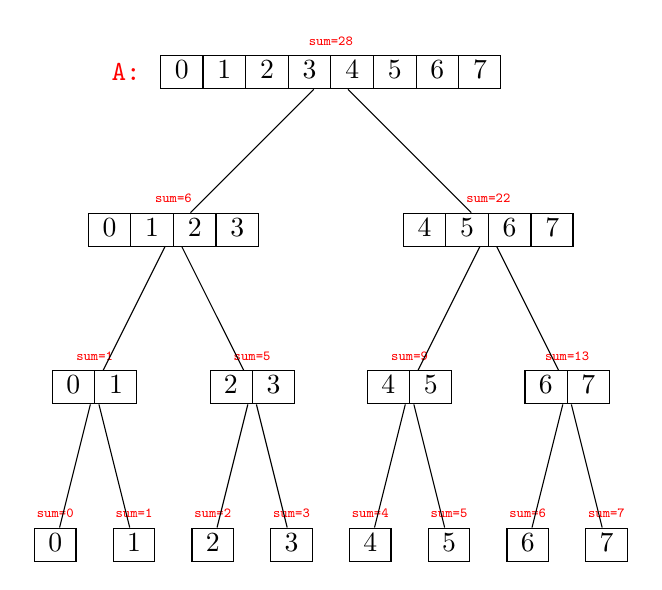
\begin{tikzpicture}
        \node at (-2.6,10) {\color{red}{\texttt{A:}}};
        \node[rectangle, draw, inner sep=+0pt,label={above:\red{sum=28}}] (root) at (0,10){
        $\begin{array}{c|c|c|c|c|c|c|c}
            0 & 1 & 2 & 3 & 4 & 5 & 6 & 7 \\
            \end{array}$};
            
        \node[rectangle, draw, inner sep=+0pt,label=\red{sum=6}] (div1) at (-2,8){
        $\begin{array}{c|c|c|c}
            0 & 1 & 2 & 3 \\
            \end{array}$};
        
        \node[rectangle, draw, inner sep=+0pt,label=\red{sum=22}] (div2) at (2,8){
        $\begin{array}{c|c|c|c}
            4 & 5 & 6 & 7  \\
            \end{array}$};
            
        \foreach \i in {0,...,3} {
            \pgfmathtruncatemacro{\first}{2*\i}
            \pgfmathtruncatemacro{\second}{2*\i+1}
            \pgfmathtruncatemacro{\s}{4*\i+1}
            \node[rectangle, draw, inner sep=+0pt,label=\red{sum=\s}] (upper\i) at (-3+\i*2,6){
                 $\begin{array}{c|c}
            \first & \second \\
            \end{array}$};
        }
            
        \foreach \i in {0,...,7} {
            \node[rectangle, draw, inner sep=+0pt,label=\red{sum=\i}] (bottom\i) at (-3.5+\i,4) {
               $\begin{array}{c}
            \i  \\
            \end{array}$};
          }
        
          \draw[-]  (root) -- (div1);
          \draw[-]  (root) -- (div2);
          \draw[-]  (div1) -- (upper0);
          \draw[-]  (div1) -- (upper1);
          \draw[-]  (div2) -- (upper2);
          \draw[-]  (div2) -- (upper3);

          \foreach \i in {0,...,3} {
            \pgfmathtruncatemacro{\left}{2*\i}
            \pgfmathtruncatemacro{\right}{2*\i+1}
            \draw[-]  (upper\i) -- (bottom\left);
            \draw[-]  (upper\i) -- (bottom\right);
          }
            
    \end{tikzpicture}
\end{document}